% TikZ Reference — Reusable Patterns for KB Explanations
%
% This file contains compilable TikZ examples for common diagram types.
% Copy and adapt these patterns in your LaTeX explanations.
% Required preamble (include in your document):
%
%   \usepackage{tikz}
%   \usetikzlibrary{arrows.meta, positioning, shapes.geometric, fit, backgrounds, calc}
%   \usepackage{amsmath, amssymb}

\documentclass[11pt]{article}
\usepackage[margin=1in]{geometry}
\usepackage{tikz}
\usetikzlibrary{arrows.meta, positioning, shapes.geometric, fit, backgrounds, calc}
\usepackage{amsmath, amssymb}

\begin{document}

% ============================================================
% CRITICAL RULES FOR ALL DIAGRAMS
% ============================================================
%
% 1. ALWAYS use `text width` (not just `minimum width`) so long text wraps.
% 2. ALWAYS use `right=` or `below=` relative positioning (not absolute `at`
%    coordinates) so nodes never overlap regardless of text length.
% 3. Keep node labels SHORT: 2-3 words max per line. Use `\\` for line breaks.
%    Bad:  "Cross-embodiment action chunks"  (will overflow)
%    Good: "Cross-Embodiment\\Action Chunks"
% 4. Use `inner sep=6pt` minimum so text doesn't touch box edges.
% 5. Spacing between nodes: `right=1.5cm` minimum (2cm preferred).

% ============================================================
% PATTERN 1: Architecture Block Diagram
% Use for: showing a single method's pipeline components
% ============================================================

\begin{figure}[h]
\centering
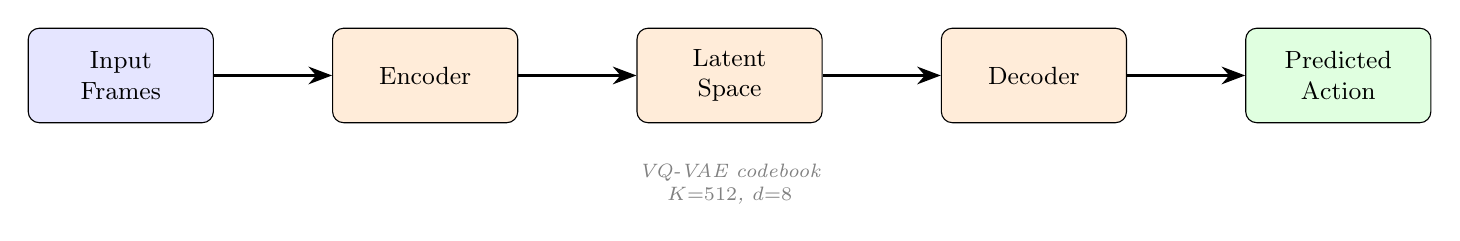
\begin{tikzpicture}[
    block/.style={rectangle, draw, rounded corners, minimum height=1.2cm,
                  text width=2cm, align=center, font=\small, inner sep=5pt},
    data/.style={block, fill=blue!10},
    model/.style={block, fill=orange!15},
    output/.style={block, fill=green!12},
    arrow/.style={-{Stealth[length=3mm]}, thick},
]
    \node[data]   (input)   {Input\\Frames};
    \node[model]  (enc)     [right=1.5cm of input]   {Encoder};
    \node[model]  (latent)  [right=1.5cm of enc]     {Latent\\Space};
    \node[model]  (dec)     [right=1.5cm of latent]  {Decoder};
    \node[output] (output)  [right=1.5cm of dec]     {Predicted\\Action};

    \draw[arrow] (input)  -- (enc);
    \draw[arrow] (enc)    -- (latent);
    \draw[arrow] (latent) -- (dec);
    \draw[arrow] (dec)    -- (output);

    % Optional: annotation below a node
    \node[below=0.4cm of latent, font=\scriptsize\itshape, text=gray, align=center]
        {VQ-VAE codebook\\ $K{=}512$, $d{=}8$};
\end{tikzpicture}
\caption{Architecture block diagram pattern.}
\end{figure}

% ============================================================
% PATTERN 2: Side-by-Side Comparison
% Use for: highlighting where two methods diverge
% Color convention: method A = blue, method B = green, shared = gray
% NOTE: Use `right=` positioning, NOT absolute `at` coordinates.
% ============================================================

\begin{figure}[h]
\centering
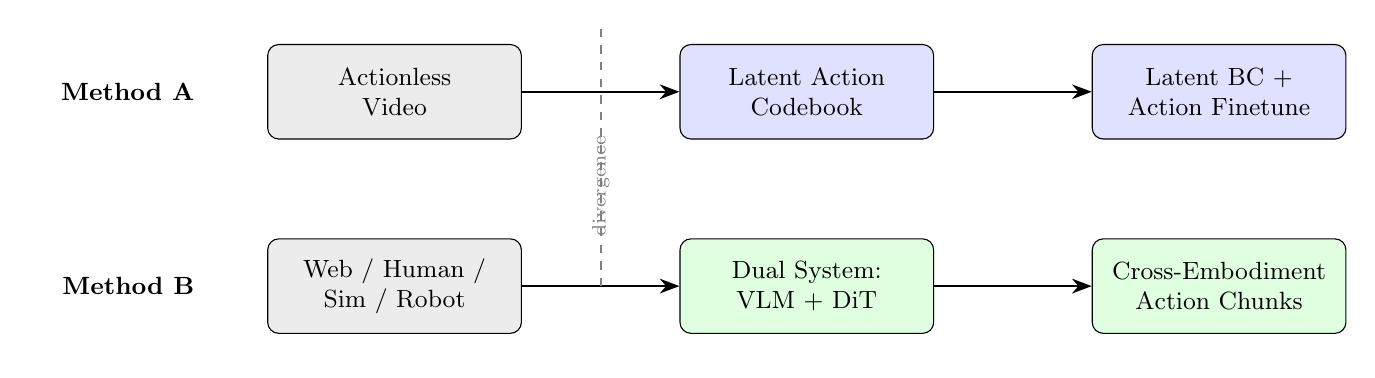
\begin{tikzpicture}[
    block/.style={rectangle, draw, rounded corners, minimum height=1.2cm,
                  text width=2.8cm, align=center, font=\small, inner sep=6pt},
    shared/.style={block, fill=gray!15},
    methodA/.style={block, fill=blue!12},
    methodB/.style={block, fill=green!12},
    arrow/.style={-{Stealth[length=2.5mm]}, thick},
    lbl/.style={font=\small\bfseries, text width=2cm, align=right},
]
    % --- Row A ---
    \node[lbl]     (lblA) {Method A};
    \node[shared]  (inA)  [right=0.8cm of lblA]  {Actionless\\Video};
    \node[methodA] (encA) [right=2cm of inA]      {Latent Action\\Codebook};
    \node[methodA] (outA) [right=2cm of encA]     {Latent BC +\\Action Finetune};

    \draw[arrow] (inA) -- (encA);
    \draw[arrow] (encA) -- (outA);

    % --- Row B (positioned below row A) ---
    \node[lbl]     (lblB) [below=2cm of lblA]     {Method B};
    \node[shared]  (inB)  [right=0.8cm of lblB]   {Web / Human /\\Sim / Robot};
    \node[methodB] (encB) [right=2cm of inB]       {Dual System:\\VLM + DiT};
    \node[methodB] (outB) [right=2cm of encB]      {Cross-Embodiment\\Action Chunks};

    \draw[arrow] (inB) -- (encB);
    \draw[arrow] (encB) -- (outB);

    % Divergence line
    \draw[dashed, gray, thick]
        ($(inA.east)!0.5!(encA.west)$) ++(0, 0.8)
        -- ($(inB.east)!0.5!(encB.west)$) ++(0, -0.8);
    \node[font=\scriptsize, text=gray, rotate=90]
        at ($(inA.east)!0.5!(encA.west) + (0,-1.2)$) {divergence};
\end{tikzpicture}
\caption{Side-by-side comparison. Shared stages in gray, method-specific in color.}
\end{figure}

% ============================================================
% PATTERN 3: Training Pipeline Flow
% Use for: showing pretraining -> finetuning -> inference stages
% ============================================================

\begin{figure}[h]
\centering
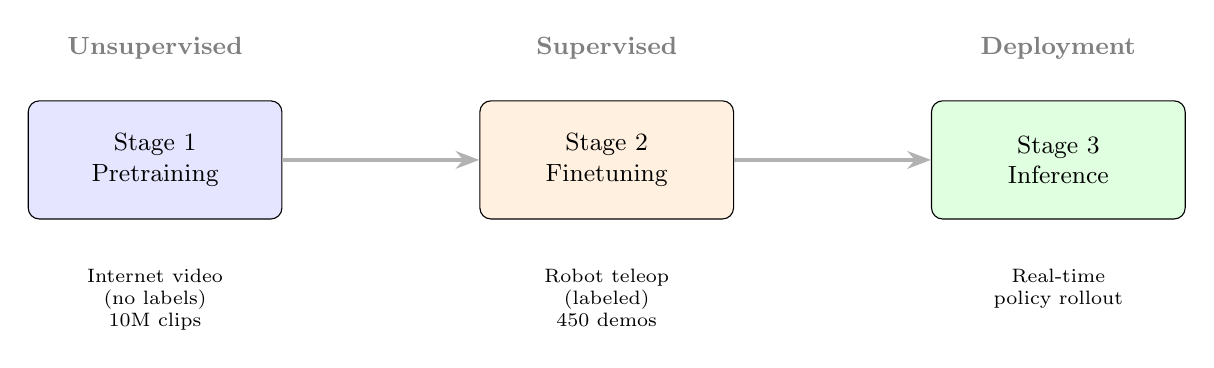
\begin{tikzpicture}[
    stage/.style={rectangle, draw, rounded corners, minimum height=1.5cm,
                  text width=2.8cm, align=center, font=\small, inner sep=6pt},
    phase/.style={font=\small\bfseries, text=gray},
    arrow/.style={-{Stealth[length=3mm]}, very thick, gray!60},
    detail/.style={font=\scriptsize, align=center},
]
    \node[stage, fill=blue!10]   (s1) {Stage 1\\Pretraining};
    \node[stage, fill=orange!12] (s2) [right=2.5cm of s1] {Stage 2\\Finetuning};
    \node[stage, fill=green!12]  (s3) [right=2.5cm of s2] {Stage 3\\Inference};

    \draw[arrow] (s1) -- (s2);
    \draw[arrow] (s2) -- (s3);

    % Details below each stage
    \node[detail, below=0.5cm of s1] {Internet video\\(no labels)\\10M clips};
    \node[detail, below=0.5cm of s2] {Robot teleop\\(labeled)\\450 demos};
    \node[detail, below=0.5cm of s3] {Real-time\\policy rollout};

    % Phase labels above
    \node[phase, above=0.4cm of s1] {Unsupervised};
    \node[phase, above=0.4cm of s2] {Supervised};
    \node[phase, above=0.4cm of s3] {Deployment};
\end{tikzpicture}
\caption{Training pipeline flow pattern.}
\end{figure}

% ============================================================
% PATTERN 4: Conceptual Diagram (Codebook Lookup)
% Use for: visualizing an abstract concept that benefits from a picture
% ============================================================

\begin{figure}[h]
\centering
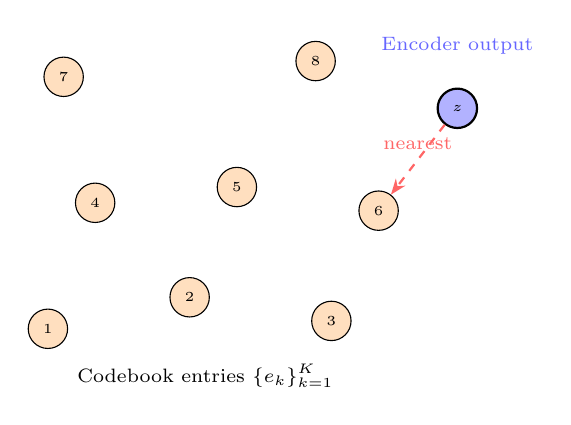
\begin{tikzpicture}[
    vec/.style={circle, draw, minimum size=0.5cm, inner sep=0pt, font=\tiny},
    entry/.style={vec, fill=orange!25},
    query/.style={vec, fill=blue!30, thick},
    arrow/.style={-{Stealth[length=2mm]}, dashed, gray},
]
    % Codebook entries — well-separated grid
    \foreach \x/\y/\label in {
        0/0/1, 1.8/0.4/2, 3.6/0.1/3, 0.6/1.6/4,
        2.4/1.8/5, 4.2/1.5/6, 0.2/3.2/7, 3.4/3.4/8}
    {
        \node[entry] (e\label) at (\x, \y) {\label};
    }

    % Query vector — clearly outside the main cluster
    \node[query] (q) at (5.2, 2.8) {$z$};

    % Nearest neighbor arrow — points to a node with clear space
    \draw[arrow, red!60, thick] (q) -- (e6)
        node[midway, above, font=\scriptsize] {nearest};

    % Labels
    \node[font=\scriptsize] at (2.0, -0.6)
        {Codebook entries $\{e_k\}_{k=1}^{K}$};
    \node[font=\scriptsize, above=0.3cm of q, blue!60]
        {Encoder output};
\end{tikzpicture}
\caption{Conceptual diagram pattern: VQ-VAE codebook nearest-neighbor lookup.}
\end{figure}

% ============================================================
% TIPS
% ============================================================
%
% - ALWAYS use `text width` on block nodes so text wraps instead of overflowing.
% - ALWAYS use relative positioning (`right=2cm of nodeA`) instead of absolute
%   coordinates (`at (4,0)`) — absolute coords cause overlaps with longer text.
% - Keep node labels to 2-3 words per line. Break with `\\`.
% - Use `inner sep=6pt` so text has padding inside the box.
% - Node spacing: 2cm minimum between nodes (use 2.5cm for pipeline flows).
% - Always include \usetikzlibrary{arrows.meta, positioning} at minimum.
% - Add more libraries as needed: shapes.geometric (diamonds, ellipses),
%   fit (bounding boxes), backgrounds (shaded regions), calc (coordinate math).
% - Keep diagrams compact: 3-8 nodes is the sweet spot.
% - Use consistent color roles: blue=input/data, orange=model/processing,
%   green=output, gray=shared/neutral.
% - For comparisons: blue for method A, green for method B, gray for shared.
% - Add \scriptsize annotations below nodes for specific numbers (dimensions,
%   dataset sizes, loss values) — this connects the diagram to the prose.
% - For multi-method comparisons, stack pipelines vertically and draw a
%   dashed vertical line at the divergence point.

\end{document}
